\paragraph{Carta de diseño para el modelo dimensional}

La carta de diseño para el modelo dimensional se utiliza para describir el proceso de diseño de un modelo dimensional
siguiendo los pasos de la metodología Hefesto. Estos pasos incluyen la selección del proceso de negocio, la declaración
del grano, la identificación de las dimensiones y sus atributos, la identificación de las tablas de hechos y sus métricas,
y el diseño del esquema dimensional. A continuación, se presenta cada uno de estos pasos.

\begin{itemize}
    \item Seleccionar el proceso de negocio:
          \begin{itemize}
              \item Identificar las pregustas del negocio.
              \item Identificar indicadores y perspectivas.
              \item Diseñar el modelo conceptual.
          \end{itemize}
    \item Declarar el grano.
    \item Identificar las dimensiones y sus atributos.
    \item Identificar las tablas de hechos y sus métricas.
    \item Diseñar el esquema dimensional
\end{itemize}

\paragraph{Seleccionar el proceso de negocio}

\paragraph{Preguntas del negocio}

El objetivo principal del sistema de reportería de incidentes delictivos es recolectar y analizar información
sobre los incidentes delictivos reportados a través de un sistema de alarma, así como detalles de los usuarios
y datos geográficos relevantes para apoyar la toma de decisiones de las autoridades policiales.

\paragraph{Identificar indicadores y perspectivas}

\begin{itemize}
    \item Determinar el número de incidentes por tipo de incidente y zona de vigilancia.
    \item Analizar la distribución de incidentes por género, discapacidad, etnia y edad de los usuarios.
    \item Identificar las zonas con mayor número de incidentes para optimizar la vigilancia policial.
\end{itemize}

\begin{longtable}{|p{5cm}|p{5cm}|}
    \caption{Indicadores y perspectivas en base las pregustas de negocio} \label{tab:indicadores-perspectivas} \\

    \hline \multicolumn{1}{|c|}{\textbf{Indicadores}} & \multicolumn{1}{|c|}{\textbf{Perspectivas}}            \\ \hline
    \endfirsthead

    \multicolumn{2}{c}%
    {{\normalfont \tablename\ \thetable{} -- continuación de la página anterior}}                              \\
    \hline \multicolumn{1}{|c|}{\textbf{Indicadores}} & \multicolumn{1}{|c|}{\textbf{Perspectivas}}            \\ \hline
    \endhead

    \hline \multicolumn{2}{|r|}{{Continua en la siguiente página}}                                             \\ \hline
    \endfoot

    \hline \hline
    \endlastfoot
    Número de incidentes                              & Tipo de Alarma                                         \\\hline
    Número de incidentes                              & Tipo de Incidente                                      \\\hline
    Número de incidentes                              & Zona de Vigilancia                                     \\\hline
    Número de incidentes                              & Género, Discapacidad, Etnia, Estado Civil              \\
\end{longtable}

\paragraph{Declarar el grano}

El grano del modelo dimensional es un único incidente delictivo reportado. Esto implica que cada registro en la
tabla de hechos representa un incidente específico.

\paragraph{Identificar las dimensiones y sus atributos}

En las Tablas \ref{tab:dimension-tiempo}, \ref{tab:dimension-usuarios}, \ref{tab:dimension-tipo-de-alarma},
\ref{tab:dimension-tipo-de-incidente} y \ref{tab:dimension-zona-de-vigilancia} se presentan las dimensiones y
sus atributos identificados para el modelo dimensional.

\begin{longtable}{|p{6cm}|p{6cm}|}
    \caption{Dimensión de tiempo con sus atributos} \label{tab:dimension-tiempo}             \\

    \hline \multicolumn{1}{|c|}{\textbf{Campo}} & \multicolumn{1}{|c|}{\textbf{Descripción}} \\ \hline
    \endfirsthead

    \multicolumn{2}{c}%
    {{\normalfont \tablename\ \thetable{} -- continuación de la página anterior}}            \\
    \hline \multicolumn{1}{|c|}{\textbf{Campo}} & \multicolumn{1}{|c|}{\textbf{Descripción}} \\ \hline
    \endhead

    \hline \multicolumn{2}{|r|}{{Continua en la siguiente página}}                           \\ \hline
    \endfoot

    \hline \hline
    \endlastfoot
    fechaID                                     & Identificador único para cada fecha        \\\hline
    fecha                                       & Fecha completa del incidente (YYYY-MM-DD)  \\\hline
    anio                                        & Año en que ocurrió el incidente            \\\hline
    mes                                         & Mes en que ocurrió el incidente            \\\hline
    día                                         & Día en que ocurrió el incidente            \\\hline
    trimestre                                   & Trimestre en que ocurrió el incidente      \\\hline
    semestre                                    & Semestre en que ocurrió el incidente       \\\hline
    hora                                        & Hora en que ocurrió el incidente           \\
\end{longtable}

\begin{longtable}{|p{6cm}|p{6cm}|}
    \caption{Dimensión de usuarios con sus atributos} \label{tab:dimension-usuarios}         \\

    \hline \multicolumn{1}{|c|}{\textbf{Campo}} & \multicolumn{1}{|c|}{\textbf{Descripción}} \\ \hline
    \endfirsthead

    \multicolumn{2}{c}%
    {{\normalfont \tablename\ \thetable{} -- continuación de la página anterior}}            \\
    \hline \multicolumn{1}{|c|}{\textbf{Campo}} & \multicolumn{1}{|c|}{\textbf{Descripción}} \\ \hline
    \endhead

    \hline \multicolumn{2}{|r|}{{Continua en la siguiente página}}                           \\ \hline
    \endfoot

    \hline \hline
    \endlastfoot
    usuarioID                                   & Identificador único del usuario            \\\hline
    género                                      & Género del usuario                         \\\hline
    discapacidad                                & Estado de discapacidad del usuario         \\\hline
    etnia                                       & Etnia del usuario                          \\\hline
    estadoCivil                                 & Estado civil del usuario                   \\\hline
    edad                                        & Edad del usuario                           \\
\end{longtable}

\begin{longtable}{|p{6cm}|p{6cm}|}
    \caption{Dimensión de tipo de alarma con sus atributos} \label{tab:dimension-tipo-de-alarma} \\

    \hline \multicolumn{1}{|c|}{\textbf{Campo}} & \multicolumn{1}{|c|}{\textbf{Descripción}}     \\ \hline
    \endfirsthead

    \multicolumn{2}{c}%
    {{\normalfont \tablename\ \thetable{} -- continuación de la página anterior}}                \\
    \hline \multicolumn{1}{|c|}{\textbf{Campo}} & \multicolumn{1}{|c|}{\textbf{Descripción}}     \\ \hline
    \endhead

    \hline \multicolumn{2}{|r|}{{Continua en la siguiente página}}                               \\ \hline
    \endfoot

    \hline \hline
    \endlastfoot
    tipoAlarmaID                                & Identificador único del tipo de alarma         \\\hline
    nombreTipoAlarma                            & Nombre del tipo de alarma                      \\
\end{longtable}

\begin{longtable}{|p{6cm}|p{6cm}|}
    \caption{Dimensión de tipo de incidente con sus atributos} \label{tab:dimension-tipo-de-incidente} \\

    \hline \multicolumn{1}{|c|}{\textbf{Campo}} & \multicolumn{1}{|c|}{\textbf{Descripción}}           \\ \hline
    \endfirsthead

    \multicolumn{2}{c}%
    {{\normalfont \tablename\ \thetable{} -- continuación de la página anterior}}                      \\
    \hline \multicolumn{1}{|c|}{\textbf{Campo}} & \multicolumn{1}{|c|}{\textbf{Descripción}}           \\ \hline
    \endhead

    \hline \multicolumn{2}{|r|}{{Continua en la siguiente página}}                                     \\ \hline
    \endfoot

    \hline \hline
    \endlastfoot
    tipoIncidenteID                             & Identificador único del tipo de incidente            \\\hline
    nombreTipoIncidente                         & Nombre del tipo de incidente                         \\
\end{longtable}

\begin{longtable}{|p{6cm}|p{6cm}|}
    \caption{Dimensión de zonas de vigilancia con sus atributos} \label{tab:dimension-zonas-vigilancia} \\

    \hline \multicolumn{1}{|c|}{\textbf{Campo}} & \multicolumn{1}{|c|}{\textbf{Descripción}}            \\ \hline
    \endfirsthead

    \multicolumn{2}{c}%
    {{\normalfont \tablename\ \thetable{} -- continuación de la página anterior}}                       \\
    \hline \multicolumn{1}{|c|}{\textbf{Campo}} & \multicolumn{1}{|c|}{\textbf{Descripción}}            \\ \hline
    \endhead

    \hline \multicolumn{2}{|r|}{{Continua en la siguiente página}}                                      \\ \hline
    \endfoot

    \hline \hline
    \endlastfoot
    zonaVigilanciaID                            & Identificador único de la zona de vigilancia          \\\hline
    polígono                                    & Representación geográfica de la zona de vigilancia    \\\hline
    nombreZonaVigilancia                        & Nombre de la zona de vigilancia                       \\
\end{longtable}

\begin{longtable}{|p{6cm}|p{6cm}|}
    \caption{Dimensión de ubicación con sus atributos} \label{tab:dimension-zonas-vigilancia} \\

    \hline \multicolumn{1}{|c|}{\textbf{Campo}} & \multicolumn{1}{|c|}{\textbf{Descripción}}  \\ \hline
    \endfirsthead

    \multicolumn{2}{c}%
    {{\normalfont \tablename\ \thetable{} -- continuación de la página anterior}}             \\
    \hline \multicolumn{1}{|c|}{\textbf{Campo}} & \multicolumn{1}{|c|}{\textbf{Descripción}}  \\ \hline
    \endhead

    \hline \multicolumn{2}{|r|}{{Continua en la siguiente página}}                            \\ \hline
    \endfoot

    \hline \hline
    \endlastfoot
    ubicacionID                                 & Identificador único de la ubicación         \\\hline
    canton                                      & Cantón del lugar del incidente              \\\hline
    ciudad                                      & Ciudad del lugar del incidente              \\
\end{longtable}

\paragraph{Identificar las tablas de hechos y sus métricas}

En la Tabla \ref{tab:hechos-incidentes-delictivos} se presentan los hechos de incidentes delictivos y sus atributos.

\begin{longtable}{|p{6cm}|p{6cm}|}
    \caption{Hechos de incidentes delictivos con sus atributos} \label{tab:hechos-incidentes-delictivos}     \\

    \hline \multicolumn{1}{|c|}{\textbf{Campo}} & \multicolumn{1}{|c|}{\textbf{Descripción}}                 \\ \hline
    \endfirsthead

    \multicolumn{2}{c}%
    {{\normalfont \tablename\ \thetable{} -- continuación de la página anterior}}                            \\
    \hline \multicolumn{1}{|c|}{\textbf{Campo}} & \multicolumn{1}{|c|}{\textbf{Descripción}}                 \\ \hline
    \endhead

    \hline \multicolumn{2}{|r|}{{Continua en la siguiente página}}                                           \\ \hline
    \endfoot

    \hline \hline
    \endlastfoot
    incidenteID                                 & Clave primaria de la tabla de hechos incidentes delictivos \\\hline
    fechaID                                     & Clave foránea a la dimensión de tiempo                     \\\hline
    usuarioID                                   & Clave foránea a la dimensión de usuarios                   \\\hline
    tipoAlarmaID                                & Clave foránea a la dimensión de tipo de alarma             \\\hline
    tipoIncidenteID                             & Clave foránea a la dimensión de tipo de incidente          \\\hline
    zonaVigilanciaID                            & Clave foránea a la dimensión de zonas de vigilancia        \\\hline
    ubicacionID                                 & Clave foránea a la dimensión de ubicación geográfica       \\\hline
    numeroIncidentes                            & Número de incidentes reportados                            \\\hline
\end{longtable}

\paragraph{Esquema dimensional}

En la Figura \ref{fig:esquema-modelo-dimensional} se muestra el esquema del modelo dimensional propuesto para el sistema de reportería de incidentes delictivos.

\begin{figure}[H]
    \centering
    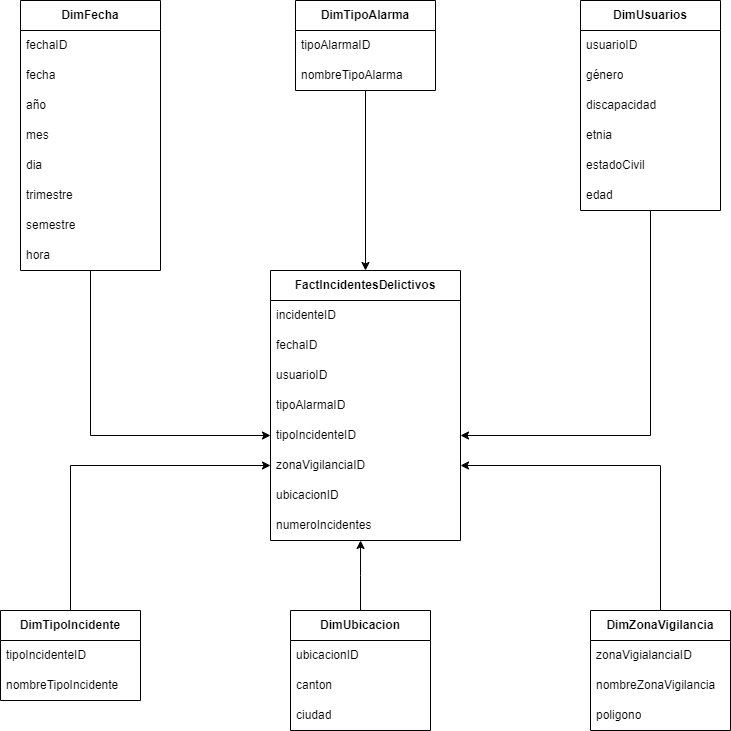
\includegraphics[width=1\textwidth]{chapters/III-resultados-y-discusion/resources/images/esquema-modelo-dimensional.png}
    \caption{Esquema del modelo dimensional para el sistema de reportería de incidentes delictivos}
    \label{fig:esquema-modelo-dimensional}
\end{figure}